\section{Figuras con pgfplots}

Ahora dibujaremos un gráfica de una función de $\mathbb{R}$ en $\mathbb{R}$

\begin{figure}[h!]
    \centering
    \begin{tikzpicture}
        \begin{axis}
        \addplot[color=red]{exp(x)};
        \end{axis}
    \end{tikzpicture}
    \caption{Caption}
    \label{fig:enter-label}
\end{figure}

Ahora una figura en $3$-D

\begin{figure}[h!]
    \centering
    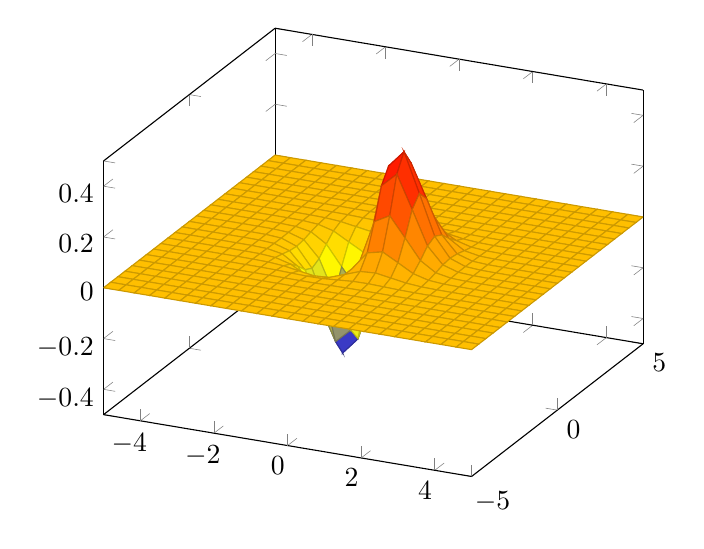
\begin{tikzpicture}
        \begin{axis}
            \addplot3[surf,]{exp(-x^2-y^2)*x};
        \end{axis}
    \end{tikzpicture}
    \caption{Caption}
    \label{fig:enter-label}
\end{figure}

\subsection{Ejemplos}

\begin{enumerate}
    \item {\bf 2D}

    \begin{figure}[h!]
        \centering
        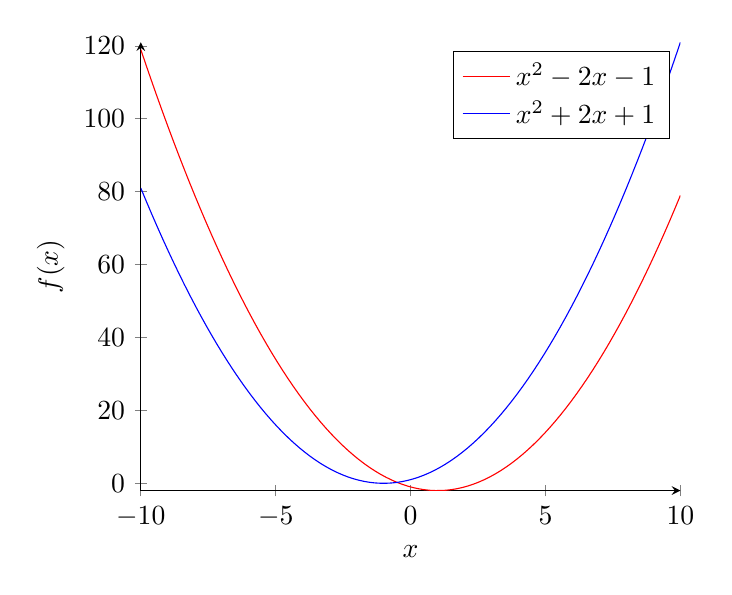
\begin{tikzpicture}
            \begin{axis}[axis lines=left,xlabel=$x$,ylabel=$f(x)$]
             \addplot[domain=-10:10,samples=100,color=red]{x^2-2*x-1};  
             \addlegendentry{$x^2-2x-1$}

             \addplot[domain=-10:10,samples=100,color=blue]{x^2+2*x+1};
             \addlegendentry{$x^2+2x+1$}
            \end{axis}
        \end{tikzpicture}
        \caption{parábolas}
        \label{fig:enter-label}
    \end{figure}

    \item Datos

    \begin{figure}[h!]
        \centering
        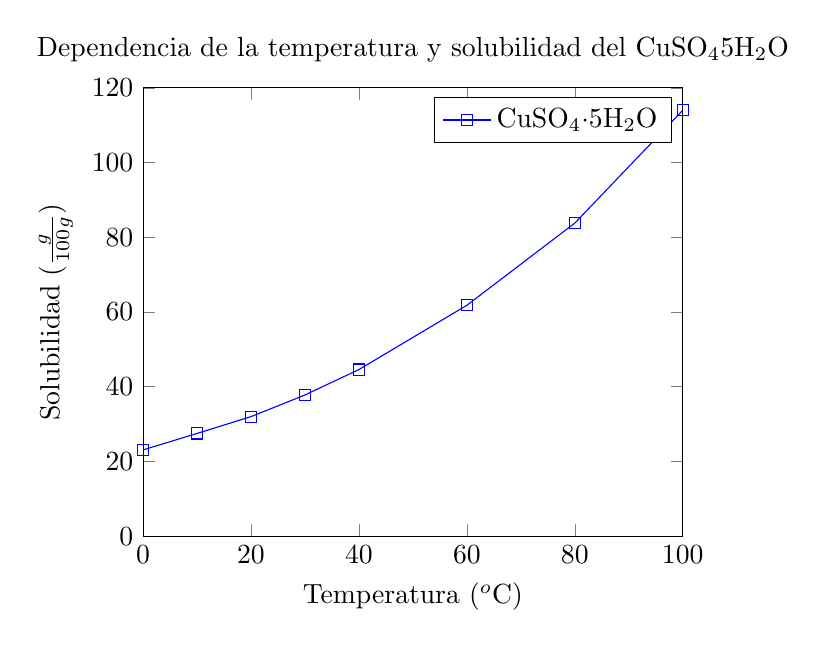
\begin{tikzpicture}
            \begin{axis}
                [
                title= Dependencia de la temperatura y solubilidad del CuSO$_4$5H$_2$O,
                xlabel=Temperatura ($^{o}$C),
                ylabel=Solubilidad ($\frac{g}{100 g}$),
                xmin=0,xmax=100,
                ymin=0,ymax=120,
                xtick={0,20,40,60,80,100},
                ytick={0,20,40,60,80,100,120},
                grid style=dashed,
                ]
                \addplot[color=blue,mark=square,] coordinates {(0,23.1)(10,27.5)(20,32)(30,37.8)(40,44.6)(60,61.8)(80,83.8)(100,114)};
                \legend{CuSO$_4\cdot$5H$_2$O}
            \end{axis}
        \end{tikzpicture}
        \caption{Caption}
        \label{fig:enter-label}
    \end{figure}

    \item Barras
    \begin{figure}[h!]
        \centering
        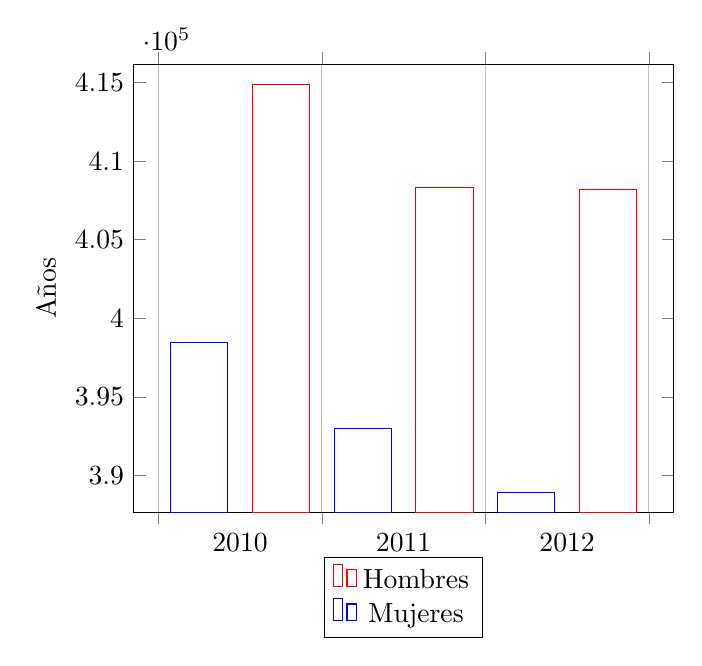
\begin{tikzpicture}
            \begin{axis}
                [
                x tick label style={/pgf/number format/1000 sep=},
                ylabel=Años,
                enlargelimits=0.05,
                legend style={at={(0.5,-0.1)},anchor=north},
                ybar interval=0.7,             
                ]
                \addplot[color=red]coordinates{(2012,408184) (2011,408348)
		 (2010,414870) (2009,412156)};
                \addplot[color=blue] coordinates{(2012,388950) (2011,393007) 
		(2010,398449) (2009,395972)};
  \legend{Hombres, Mujeres}
            \end{axis}
        \end{tikzpicture}
        \caption{Caption}
        \label{fig:enter-label}
    \end{figure}

    \item 3D
    \begin{figure}[h!]
        \centering
        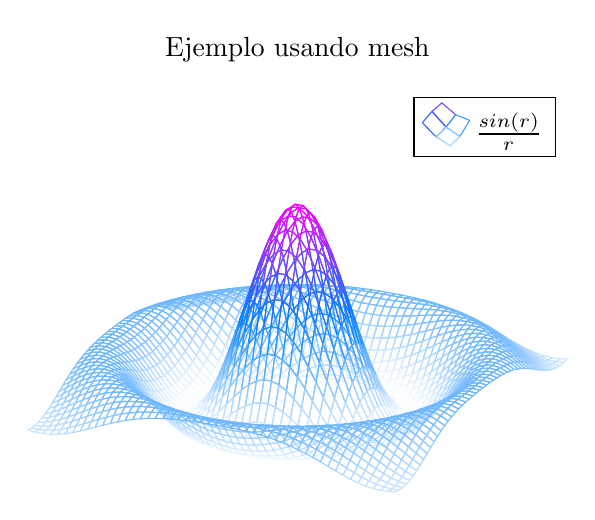
\begin{tikzpicture}
            \begin{axis}
                [
                title=Ejemplo usando mesh,
                hide axis,
                colormap/cool,
                ]
            \addplot3[mesh,samples=50,domain=-8:8,]{sin(deg(sqrt(x^2+y^2)))/sqrt(x^2+y^2)} ;
            \addlegendentry{\(\frac{sin(r)}{r}\)}
            \end{axis}
        \end{tikzpicture}
        \caption{Caption}
        \label{fig:enter-label}
    \end{figure}

    \item Contour con gnuplot
    \begin{figure}
        \centering
        \begin{tikzpicture}
\begin{axis}
[
    title={Contour plot, view from top},
    view={0}{90}
]
\addplot3[
    contour gnuplot={levels={0.8, 0.4, 0.2, -0.2}}
]
{sin(deg(sqrt(x^2+y^2)))/sqrt(x^2+y^2)};
\end{axis}
\end{tikzpicture}
        \caption{Caption}
        \label{fig:enter-label}
    \end{figure}
\end{enumerate}

\begin{wrapfigure}{r}{0.25\textwidth}
    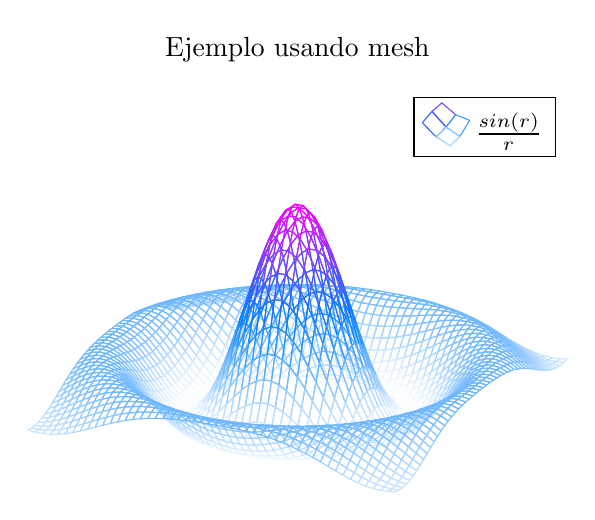
\begin{tikzpicture}
            \begin{axis}
                [
                title=Ejemplo usando mesh,
                hide axis,
                colormap/cool,
                ]
            \addplot3[mesh,samples=50,domain=-8:8,]{sin(deg(sqrt(x^2+y^2)))/sqrt(x^2+y^2)} ;
            \addlegendentry{\(\frac{sin(r)}{r}\)}
            \end{axis}
        \end{tikzpicture}
\end{wrapfigure}

Este texto esta alrededor de la imagen que hicimos en el penúltimo ejemplo, orientada del lado derecho de nuestro escrito.

\begin{wrapfigure}{l}{0.25\textwidth}
\begin{tikzpicture}
\begin{axis}
[
    title={Contour plot, view from top},
    view={0}{90}
]
\addplot3[
    contour gnuplot={levels={0.8, 0.4, 0.2, -0.2}}
]
{sin(deg(sqrt(x^2+y^2)))/sqrt(x^2+y^2)};
\end{axis}
\end{tikzpicture}
\end{wrapfigure}

